\chapter{Experimenty DOSIS a DOSIS 3D}
Informace v této kapitole byly čerpány převážně ze zdrojů \cite{dosis,dosis2}.

Experiment DOSIS (Dose Distribution Inside the ISS, distribuce dávky uvnitř ISS) probíhal v letech 2009-2011, experiment DOSIS3D probíhá od roku 2012. Jejich cílem je vyšetření prostorové distribuce dávky v modulu ISS Columbus a získání dat, která by vedla k vytvoření 3D modelu rozložení dávek/dávkového ekvivalentu.
%a DOSIS 3D probíhají roku 2009 za účelem vyšetření prostorové distribuce dávky v modulu ISS Columbus. Kýženým cílem bylo získání dat, která by vedla k vytvoření 3D modelu této distribuce.

Na experimentech se podílí řada institucí z různých zemí, jejich přehled je v tab.~\ref{tab:dosis_instituce}. Hlavním koordinátorem je DLR. MTA EK byla v průběhu experimentu přejmenována na AERI, v této práci je využívána původní zkratka. %formulací si nejsem jist
\begin{table}[H]
  \centering
\renewcommand{\baselinestretch}{0.8}
\renewcommand{\arraystretch}{2}
\footnotesize
\caption{Organizace podílející se na experimentech DOSIS a DOSIS3D. \cite{dosis}}
  \label{tab:dosis_instituce}
  \begin{tabularx}{\textwidth}{X}
    \toprule
German Aerospace Center (DLR), Institute of Aerospace Medicine, Linder Höhe, 51147 Köln, Germany\\
Christian Albrechts Universität zu Kiel (CAU), Christian-Albrechts-Platz, 24118 Kiel, Germany                                    \\
Institute of Nuclear Physics, Polish Academy of Sciences (IFJ), PL-31342 Krakow, Poland                                          \\
International Atomic Energy Agency (IAEA), Division of Radiation, Transport and Waste Safety, 1400 Vienna, Austria               \\
Technische Universität Wien, Atominstitut (ATI), Stadionallee 2, 1020 Vienna, Austria                                            \\
EGB MedAustron, Marie-Curie-Straße 5, 2700 Wiener Neustadt, Austria                                                              \\
Centre for Energy Research, (MTA EK/AERI), Konkoly Thege ut 29-33, 1121 Budapest, Hungary                                             \\
Nuclear Physics Institute of the CAS (NPI), Department of Radiation Dosimetry, Na Truhlarce 39/64, 180 00 Prague, Czech Republic \\
Belgian Nuclear Research Center (SCK$\cdot$CEN), Boeretang 200, 2400 Mol, Belgium    \\
NASA, Space Radiation Analysis Group (NASA/SRAG), Houston, TX 77058, USA       \\
Leidos, Exploration \& Mission Support, 2400 NASA Pkwy, Houston, TX 77058, USA  \\
Physics Department, Oklahoma State University (OSU), Stillwater, OK 74078, USA \\
National Institute of Radiological Sciences (NIRS), National Institutes for Quantum and Radiological Science and Technology (QST), 4-9-1 Anagawa, Inage, 263-8555 Chiba, Japan\\
OHB System AG, Universitätsallee 27-29, 28359 Bremen, Germany\\
\bottomrule
  \end{tabularx}
\end{table}

Měření byla, respektive jsou prováděna pasivními a aktivními detektory, které jsou pevně umístěny v modulu Columbus. Pasivní detektory zajišťují určení prostorové distribuce dávky a dlouhodobého vývoje pole záření, aktivní naopak slouží k určení změn pole záření v čase. V případě aktivních detektorů se jedná o dva detektory DOSTEL (DOSimetry TELescope). V dalším textu se budeme zabývat pouze pasivními detektory.

\section{Rozmístění pasivních detektorů}
V rámci experimentu DOSIS, resp. DOSIS3D je v modulu Columbus rozmístěno jedenáct PDP (Passive Detector Packages, balíčky pasivních dektorů), které obsahují termoluminiscenční detektory (TLD, thermoluminescent detectors), detektory využívající optickou stimulaci (OSLD, optically stimulated luminescent detectors) a detektory stop v pevné fázi (TED, nuclear track etched detectors). Na obr. \ref{fig:columbus_rozmisteni} vidíme rozmístění PDPs; pět z nich je umístěno na čelní stěně, dalších šest na zadní stěně. Jedenáctý balíček označený symbolem X, též označovaný jako Triple PDP (trojitý PDP), je umístěn blízko aktivních detektorů a pokrývá větší plochu než ostatní PDPs. Osm PDPs je umístěno ve skříňových modulech (viz oddíl \ref{sec:ISS_columbus}); více informací o umístění pasivních detektorů je k dostání v \cite{dosis}. %další obrázek???
\begin{figure}[h]
  \centering
  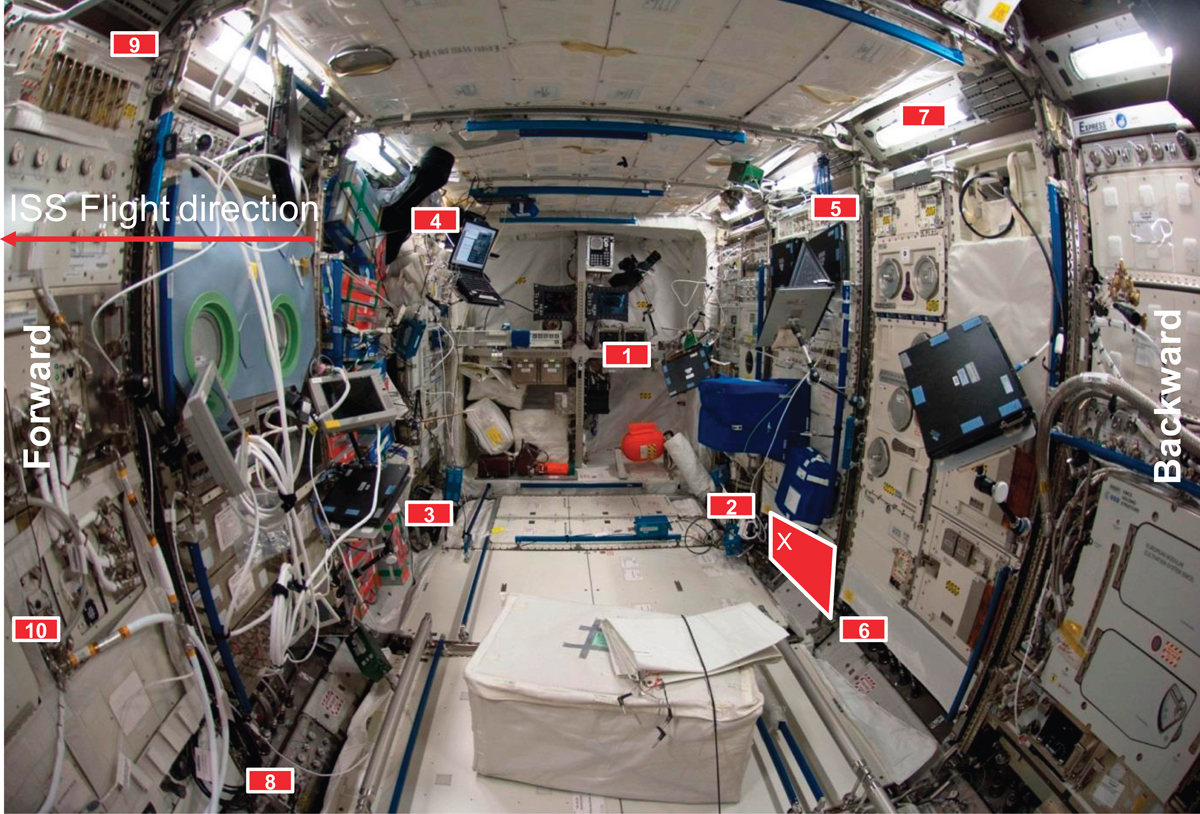
\includegraphics[width=\textwidth]{columbus_rozmisteni.jpg}
  \caption{Rozmístění jedenácti balíčků s pasivními detektory v modulu Columbus; jedenáctý je označen symbolem X a v jeho blízkosti jsou umístěny i aktivní detektory. Obrázek dále obsahuje šipku ukazující směr letu. \cite{dosis}}
  \label{fig:columbus_rozmisteni}
\end{figure}

\section{Průběh experimentů}%mozna DOPLNIT:DOSTEL-1 meril kratsi dobu nez DOSTEL-2!!!!!!!!!!!!!
Experiment DOSIS probíhal mezi lety 2009 a 2011. Doba trvání experimentu DOSIS3D byla původně stanovena na rozmezí let 2012-2016, avšak v roce 2016 byla prodloužena a experiment stále běží. V rámci těchto experimentů bylo v modulu Columbus zatím k dnešnímu datu (13. 5. 2017) postupně upevněno 10 sad pasivních detektorů (DOSIS -- dvě sady, DOSIS3D -- devět sad) a na květen/červen 2017 se plánuje upevnění jedenácté. Každá sada obsahovala obsahovala výše zmíněných 11 PDPs. V tab.~\ref{tab:dosis_timeline} je vidět časový vývoj v obměně prvních osmi sad a aktivních detektorů (ty byly u obou experimentů pouze dva, DOSTEL-1 a DOSTEL-2), tab.~\ref{tab:dosis_timeline_passive} pak obsahuje podrobnější informace o pasivních detektorech (dopravení na ISS, instalaci, doba používání, ukončení měření, návrat na Zem, nadmořská výška); sady 7, 8, 9 experimentu DOSIS3D jsou stále
vyhodnocovány, proto u nich není v tabulce údaj o nadmořské výšce; sada 10 není zatím vyhodnocena vůbec. 

První z experimentů započal 15. července 2009 startem raketoplánu Endeavor, na jehož palubě byla
první sada pasivních detektorů spolu s aktivními detektory \mbox{DOSTEL-1,2}. Jeho část skládající se z měření pasivními detektory skončila 26. května 2010 návratem druhé sady. Experiment DOSIS3D započal 15. května 2012 startem lodi Soyuz 30S. 
\begin{table}[H]
  \centering
  \caption{Vývoj experimentů DOSIS a DOSIS3D v čase. Číslo na svislé ose označuje $n$-tou sadu pasivních detektorů, písmeno A značí aktivní detektor. \cite{dosis}}
  \label{tab:dosis_timeline}
  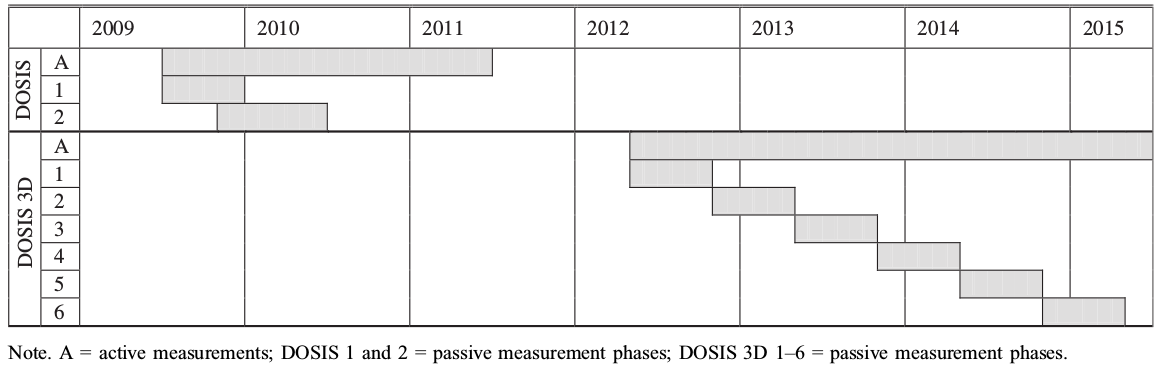
\includegraphics[width=\textwidth]{dosis_timeline}
\end{table}
\begin{table}[H]
  \centering
\footnotesize
  \caption{Časový vývoj používaných sad pasivních detektorů. Tabulka dále obsahuje dobu, kterou daná sada strávila na misi (tj. od startu do návratu na Zem), v závorce je doba, po kterou pasivní detektory měřily; pokrytí je podíl těchto dvou dob. Poslední sloupec obsahuje rozmezí nadmořské výšky, ve které se ISS v daný časový úsek nacházela~\cite{dosis}. Sady 7, 8 a 9 experimentu DOSIS3D nebyly ještě zcela vyhodnoceny (květen 2017), sada 10 nebyla téhož experimentu nebyla vyhodnocena vůbec.}
  \label{tab:dosis_timeline_passive}
  \begin{tabularx}{\textwidth}{llllll}
	\toprule
	&Sada&	Počátek-konec	&Doba trvání [dny]	&Pokrytí [\%]	&Nadmořská výška ISS [km]\\
	\midrule
DOSIS	&1	&Červenec 2009-	&136 (127)	&93,3	&339-348\\
		&	&Listopad 2009	&		    &       &       \\
		&2	&Listopad 2009-	&191 (178)	&93,2	&337-349\\
		&	&Květen 2010	&		    &       &       \\
DOSIS3D	&1	&Květen 2012-	&125 (113)	&90,4	&397-417\\
		&	&Září 2012		&	        &       &       \\
		&2	&Říjen 2012-	&144 (137)	&95,1	&407-416\\
		&	&Březen 2013	&		    &       &       \\
		&3	&Březen 2013-	&167 (156)	&93,4	&407-416\\
		&	&Září 2013		&	        &       &       \\
		&4	&Září 2013-		&167 (156)	&93,4	&413-418\\
		&	&Březen 2014	&		    &       &       \\
		&5	&Březen 2014-	&170 (161)	&94,4	&407-416\\
		&	&Září 2014		&	        &       &       \\
		&6	&Září 2014-		&167 (161)	&96,4	&413-418\\
		&	&Březen 2015	&			&		&		\\
		&7	&Březen 2015-	&259 (256	&98,8	&		\\
		&	&Prosinec 2015	&			&		&		\\
		&8	&Prosinec 2015- &186 (180)	&96,8	&		\\
		&	&Červen 2016	&			&		&		\\
		&9	&Červenec 2016	&115 (109)	&94,8	&		\\
		&	&Říjen 2016		&			&		&		\\
		\bottomrule
  \end{tabularx}
  %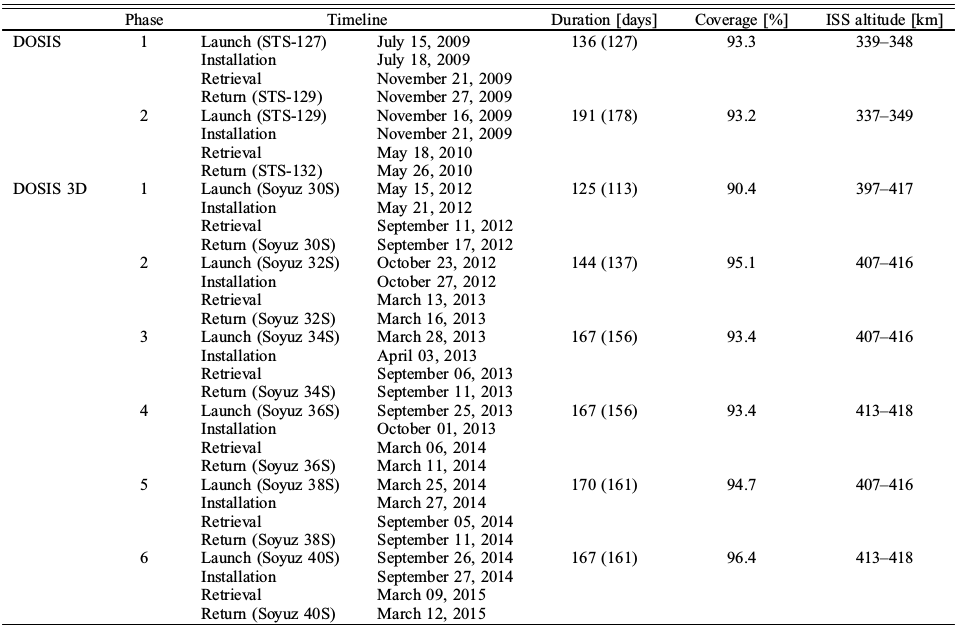
\includegraphics[width=\textwidth]{dosis_timeline_passive}
\end{table}
\subsection{Vývoj nadmořské výšky a slunečního cyklu}\label{sec:dosis_altitudeSlunecniCyklus} %špatné odsazení
Naměřená data jsou ovlivněna řadou parametrů. Nadmořská výška a fáze slunečního cyklu jsou jedny z nejvýznamnějších. 

Na obr. \ref{subfig:dosis_altitude} je znázorněn časový vývoj nadmořské výšky ISS. Pro DOSIS nadmořská výška nabývala hodnot z intervalu [337, 375] km, pro DOSIS3D nabývala hodnot z intervalu [398, 417] km. V obrázku lze vypozorovat prudký nárůst z cca 340 km do 375 km, který se udál ke konci experimentu DOSIS; tehdy již měřily pouze aktivní detektory. Změna nadmořské výšky ovlivňuje ozáření stanice (viz oddíl \ref{sec:kosmickeZareni_altitude}). 

Z informací v oddílu \ref{sec:kosmickeZareni_solar} plyne, že za slunečního maxima je obdržená dávka nejmenší a naopak za slunečního minima největší (za předpokladu stálosti ostatních parametrů ovlivňujících velikost obdržené dávky). To je znázorněno na obr. \ref{subfig:dosis_solarCycle}, kde je zobrazena závislost četnosti detekovaných neutronů na čase (počet detekovaných neutronů klesá s rostoucí sluneční aktivitou). Experiment DOSIS probíhal za slunečního minima (2009 až 2011) a naopak experiment DOSIS3D probíhal za slunečního maxima, které nastalo v letech 2013 a 2014.   
\begin{figure}[h]
  \centering
  \begin{subfigure}{0.45\textwidth}
    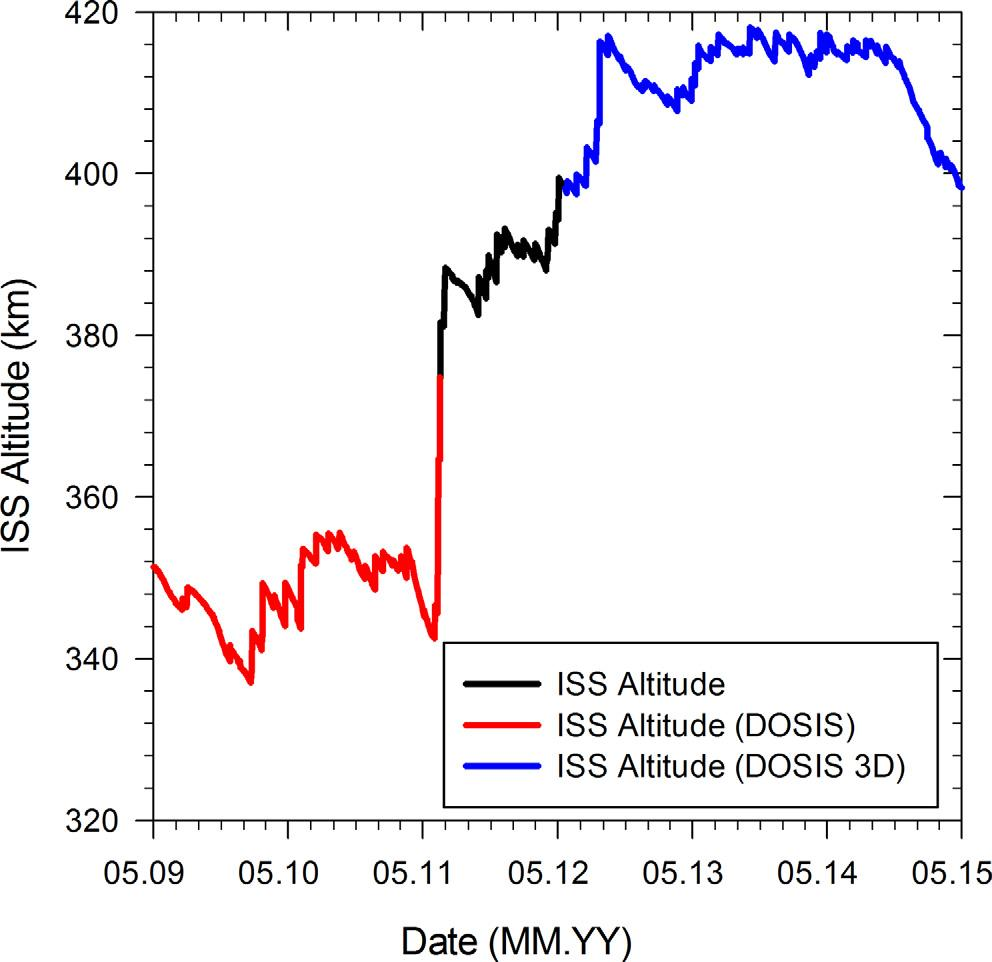
\includegraphics[width=\textwidth]{dosis_altitude.jpeg}
    \caption{}
    \label{subfig:dosis_altitude}
  \end{subfigure}
  \begin{subfigure}{0.45\textwidth}
    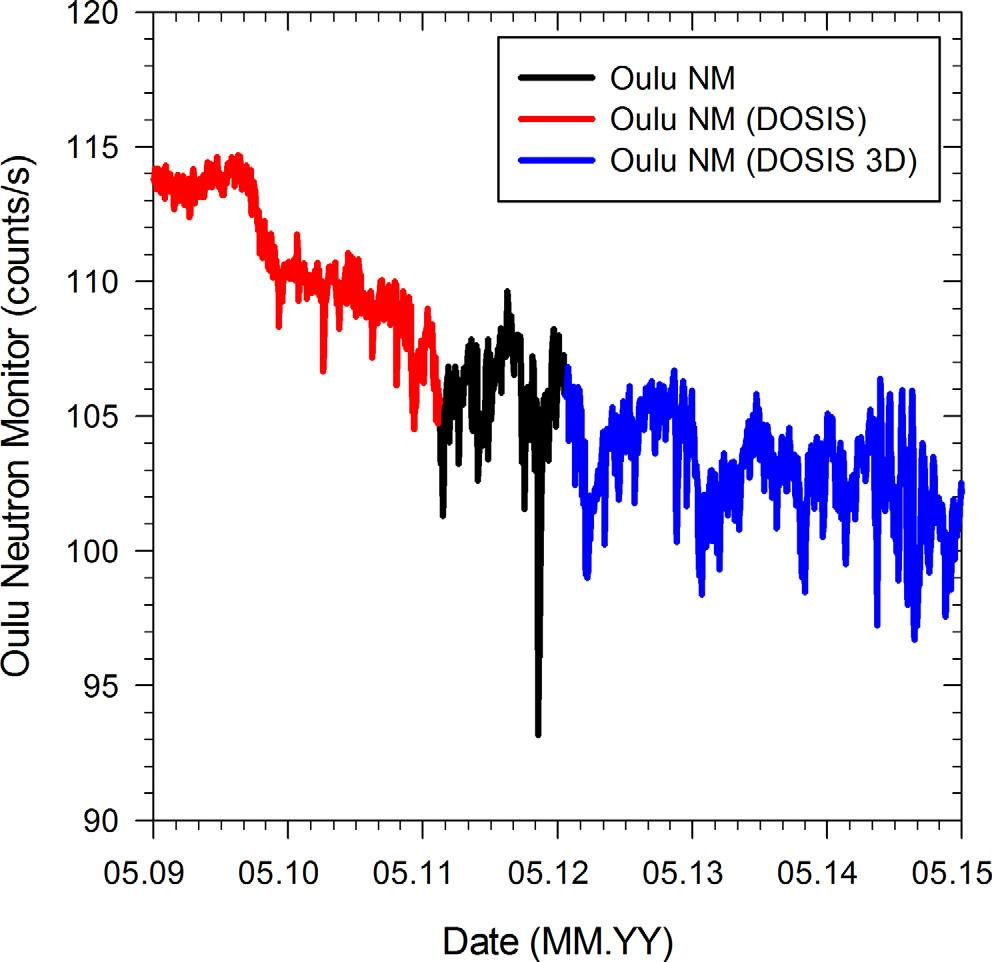
\includegraphics[width=\textwidth]{dosis_solarCycle.jpeg}
    \caption{}
    \label{subfig:dosis_solarCycle}
  \end{subfigure}
  \caption{V (a) je časový vývoj nadmořské výšky ISS: červeně je vyznačen vývoj v rámci DOSIS, modře v rámci DOSIS3D; černě je označen vývoj nadmořské výšky v době, kdy neprobíhal žádný z experimentů. V (b) je naměřená četnost Oulu neutronovým monitorem, značení je stejné jako v (a); klesající vývoj četnosti impulzů značí rostoucí sluneční aktivitu. \cite{dosis,dosis_oulu}} 
  \label{fig:dosis_parameters}
\end{figure}

\section{Používané detektory}%AKTUALNOST TABULEK?????!!!!!!!!!!!!!!!
Tento oddíl pojednává o používaných detektorech v experimentech DOSIS a DOSIS3D. Podrobnější informace o pasivních detektorech (např. jak probíhá měření absorbované dávky a dávkového ekvivalentu; srovnání jednotlivých typů pasivních detektorů) jsou v kapitole \ref{sec:detektory_detektory}. O aktivních detektorech tato práce nepojednává, podrobnější informace lze dohledat v \cite{activeDetectors,dosis2}.

%V případě pasivních detektorů jsou principy a fungování detektorů a potažmo i témata jako využívané kombinace detektorů pro měření absorbované dávky a dávkového ekvivalentu, srovnání pasivních detektorů mezi sebou a s aktivními detektory zpracována v kapitole \ref{sec:detektory_detektory}. V případě 

V experimentech DOSIS a DOSIS3D jsou používány následující tři typy pasivních detektorů: termoluminiscenční detektory (TLD), opticky stimulované luminiscenční detektory (OSLD) a detektory stop v pevné fázi (TED). V aktivní složce měření je využívána detektorová jednotka DOSTEL. 

Na konci tohoto oddílu je podrobný přehled detektorů, které používá NPI, tj. Ústav jaderné fyziky AVČR, oddělení dozimetrie záření.
\subsection{Termoluminiscenční detektory}
Používané TL detektory jsou v tabulce~\ref{tab:dosis_pouzivaneTLD}. Ta obsahuje název instituce spolu s názvy a materiály TLD, které jsou danými institucemi používány. Avšak to pro důkladný popis daného TL detektoru nestačí. Je potřeba dodat následující parametry: čtecí systém (jímž jsou detektory vyhodnocovány), jak dlouho a při jaké teplotě probíhá annealing, rychlost zahřívání, zda-li se detektor před vyhodnocením předehřívá, rychlost chlazení, kalibrační metoda a zdroj, vyhodnocení vyhřívací křivky. Lomítko v názvu TLD (v tab. \ref{tab:dosis_pouzivaneTLD}) značí dva různé TLD lišící se pouze nuklidem v materiálu: TLD-600 a MTS-6 je označení pro $^6$LiF:Mg,Ti; TLD-700 a MTS-7 pro $^7$LiF:Mg,Ti; MCP-6 pro $^6$LiF:Mg,Cu,P; MCP-7 pro $^7$LiF:Mg,Cu,P. %, tato dvojice má jinak stejné parametry. Naopak je-li nějaký materiál uveden u dvou zcela odlišně pojmenovaných TLD, pak se tyto dva TLD liší alespoň v jednom parametru.
\begin{table}[H]
  \def\arraystretch{0.8}
  \centering
  \caption{TL detektory používané různými institucemi.}
  \label{tab:dosis_pouzivaneTLD}
  \begin{tabular}{lll}
	\toprule
Institut&Název TLD&Materiál TLD\\
\midrule
DLR			 &TLD-600/700  &LiF:Mg,Ti\\
			 &TLD-300	   &CaF$_2$:Tm\\
ATI			 &TLD-600/700  &LiF:Mg,Ti\\
			 &TLD-300	   &CaF$_2$:Tm\\
IFJ			 &MTS-6/7	   &LiF:Mg,Ti\\
			 &MCP-7		   &LiF:Mg,Cu,P\\
SCK$\cdot$CEN&MTS-6/7	   &LiF:Mg,Ti\\
			 &MCP-6/7	   &LiF:Mg,Cu,P\\
MTA EK		 &MTS-6/7	   &LiF:Mg,Ti\\
NIRS		 &TLD-100	   &LiF:Mg,Ti\\
NASA/SRAG	 &TLD-100	   &LiF:Mg,Ti\\
			 &TLD-300	   &CaF$_2$:Tm\\
NPI			 &Al$_2$O$_3$:C&Al$_2$O$_3$:C\\
			 &CaSO$_4$:Dy  &CaSO$_4$:Dy\\
	\bottomrule
  \end{tabular}
\end{table}
\subsection{Opticky stimulované luminiscenční detektory}
Detektory založené na opticky stimulované luminiscenci využívají následující instituce: OSU, SCK$\cdot$CEN, NASA/SRAG, NIRS. Jsou vyrobené z jednoho materiálu (Al$_2$O$_3$:C), avšak liší se v následujících parametrech: čtecí systém, příkon energie působící na na centimetr čtvereční detektoru, filtr, doba stimulace, kalibrační metoda a kalibrační zdroj, vyhodnocení OSL křivky. Všechny tyto parametry jsou pro detektory od jednotlivých institucí v tab. 6 v \cite{dosis}. 
%nedělat tabulku, vypsat instituce normálně; ze je to jeden materiál (Al$_2$O$_3$:C), ale různé parametry; jejich vyhodnocování probíhá pomocí referenčního zdroje (ten vztah asi nepsat); to je asi vše, bude to krátké
\subsection{Detektory stop v pevné fázi}
Všechny používané detektory stop v pevné fázi jsou CR-39. V tab. \ref{tab:dosis_pouzivaneTED} jsou uvedeny instituce, které TED využívají; tabulka také obsahuje výrobce daného TED. Důležitými parametry jsou: doba leptání; teplota, při níž leptání probíhá; koncentrace NaOH, jímž se leptalo; odleptaná vrstva; analyzovaná plocha.
\begin{table}[h]
  \def\arraystretch{0.8}
  \centering
  \caption{Přehled institucí používající TED, u každé instituce jsou uvedeny výrobci příslušného detektoru.}
  \label{tab:dosis_pouzivaneTED}
  \begin{tabular}{ll}
	\toprule
	Institut& Výrobce/Jméno TED\\
	\midrule
	DLR&ATP\\
	MTA EK&TASTRAK\\
	NPI&HARZLAS TD-1\\
	IPF&TASTRAK\\ 
	NIRS&HARZLAS TD-1\\
		&TechnoTrak\\
	NASA/SRAG&ATP\\
	\bottomrule
  \end{tabular}
\end{table}

%dát sem tu tabulku celou; CR-39; velmi záleží na hardwaru (mikroskop, kamera) a softwaru!!!
%pozn.: principy, z čeho co je a proste vše podrobnější si nechat do další kapitoly
\subsection{Aktivní detektory DOSTEL}
Detektorová jednotka DOSTEL se skládá z dvou křemíkových planárních detektorů s plochou  6,94 cm$^2$ a tloušťkou 315 $\mu$m. Tyto detektory jsou od sebe vzdálené 15 mm a jsou nastaveny ve stejné geometrii jako teleskop. Jednotka může pracovat buď v dávkovém módu (``dose mode''), nebo v teleskopickém/LET módu. V prvním případě se měří četnost nárazů a dávkový příkon, v druhém LET (při náhodném nárazu do obou detektorů se měří délka doletu částice). Z naměřených dat lze určit absorbovanou dávku a dávkový ekvivalent. DOSTEL dokáže zaznamenávat částice s LET v rozsahu 0,5--400 kev/$\mu$m \cite{activeDetectors}. 

V modulu Columbus jsou nainstalovány dvě jednotky DOSTEL v navzájem kolmém směru, což umožňuje získat informace o směrovosti pole záření v modulu. Navíc díky dlouhodobosti měření DOSTEL detektory je možné studovat změny v ozáření během jedenáctiletého slunečního cyklu.

Na obrázku \ref{fig:dosis_activeDetectors} je mimo jiné vidět DOSTEL. Informace v tomto oddíle byly brány z \cite{dosis,activeDetectors}. 
\begin{figure}[H]
  \centering
  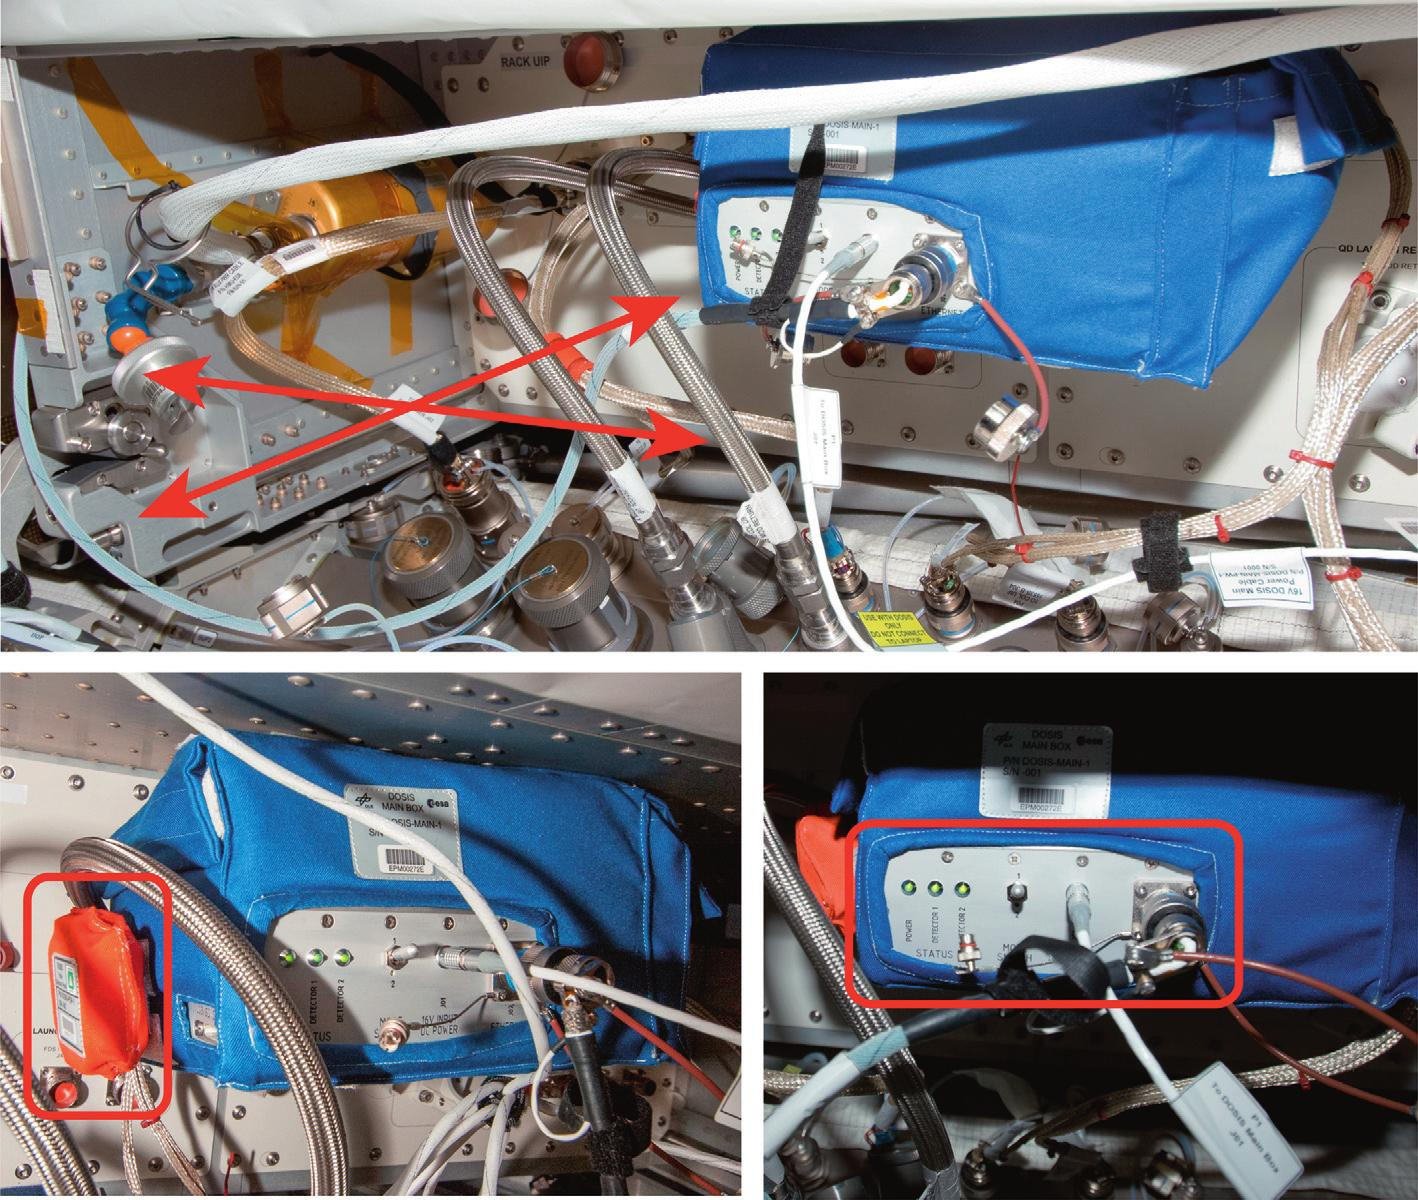
\includegraphics[width=0.8\textwidth]{dosis_activeDetectors.jpg}
  \caption{V horním obrázku je vidět modrý box, v němž jsou umístěny oba dva DOSTEL detektory; šipky ukazují namíření detektorů. Vlevo dole je vidět označený PDP připojený v blízkosti aktivních detektorů, vpravo dole je ukázáno ovládání jednoho DOSTELu. \cite{dosis2}}
  \label{fig:dosis_activeDetectors}
\end{figure}

\subsection{Detektory používané NPI}
NPI používá dva TL detektory, Al$_2$O$_3$:C a CaSO$_4$:Dy. Oba dva jsou vyhodnocovány pomocí čtecího systému RA’94 (THORN EMI 9789 QB)+TOLEDO 654 TLD Reader; rychlost zahřívání u obou je rovna 10 $^{\circ}$C/s; první není předehříván, druhý je předehříván na 150 $^{\circ}$C (22 s); annealing probíhá 20 minut za 700 $^{\circ}$C (Al$_2$O$_3$:C), respektive 10 minut za 380 $^{\circ}$C (CaSO$_4$:Dy); ochlazovací rychlost je vysoká u obou; kalibrování probíhá u obou pomocí $^{137}$Cs; u obou je vyhodnocována plocha pod vyhřívací křivkou. Oba dva mají průměr roven 5 mm a tloušťku rovnou 1 mm.


Z TED používá NPI HARZLAS TD-1 a od roku 2016 i TASTRAK. HARZLAS TD-1 je leptán 18 hodin za teploty 70 $^{\circ}$C v 5 N koncentrovaném roztoku NaOH; odleptaná vrstva je tlustá 15,3 $\mu$m. Celkově je analyzována plocha o velikosti 0,09 cm$^2$. Detektor je tlustý 0.9 mm. TASTRAK se leptá dvoufázově: první fáze trvá 6 hodin a jsou při ní zobrazeny stopy vytvořené částicemi s velkým LET; při druhé fázi, která trvá dalších 9 hodin, se zobrazí i stopy pocházejících od částic s nižším LET. Celkový čas leptání je tedy 15 hodin. Buď se postupuje postupným leptáním (6 hodin leptání, vyhodnocení, 9 hodin leptání, vyhodnocení), nebo se část detektoru leptá 6 hodin a část 15 hodin, tudíž
detektor lze vyhodnotit najednou. Detektor se leptá při 70 $^{\circ}$C v 6,25 N koncentrovaném roztoku NaOH, odleptaná vrstva je tlustá 8,04/20,1 $\mu$m; analyzuje se plocha o velikost 0,5 cm$^2$ (v obou případech). Po leptání následuje u obou detektorů nasnímání stop lineárním snímacím zařízením s vysokým rozlišením (které je součástí mikroskopu HSP-1000, \cite{dosis_HSP1000}), poté jsou snímky se stopami analyzovány programem HspFit.

TASTRAK původně využívaný pouze MTA EK začíná být používán i ostatními organizacemi, jelikož různorodost využívaných TED a jejich způsobů vyhodnocení komplikuje vzájemné porovnávání a interpretaci naměřených dat \cite{cesky}. 
%To. že nám (NPI) vyšla kalibrační krivka jinak než těm madarum, tak to psat do casti o detektorech

Informace byly brány z \cite{dosis}.

\section{Výsledky}
Zde jsou uvedeny výsledky publikované v \cite{dosis}. Jedná se o data naměřená TL a OSL detektory z obou sad DOSIS a z prvních šesti sad DOSIS3D, tedy o data naměřená mezi lety 2009 a 2015. Pro větší názornost jsou zde uvedeny i obrázky z \cite{dosis2}, které byly získány z dat naměřených aktivními detektory. 

Na naměřená data lze pohlížet z několika hledisek. Nejprve je uvedeno srovnání dat získaných z několika TL a ze všech OSL detektorů v rámci jedné sady experimentu DOSIS3D, konkrétně druhé. Poté následuje srovnání dat, které byly získány TL detektory $^6$LiF:Mg,Ti a $^7$LiF:Mg,Ti v rámci všech osmi vyhodnocených sad. Dále je zmíněno stručné porovnání dat z pasivních a aktivních detektorů; nakonec je uvedeno krátké srovnání s daty naměřenými mimo modul Columbus. 

Srovnáním dat od TL detektorů z DOSIS3D s daty získanými v ISS mimo modul Columbus od detektorů stejného materiálu plyne, že velmi závisí na lokálním stínění. Data se v závislosti na jeho tloušťce mohou lišit až dvojnásobně.  

%Vzhledem k tomu, že tato práce je primárně zaměřena na detektory stop v pevné fázi, tak jsou informace v tomto oddíle značně povrchní. %MOZNA ZMENIT?!!!!
Tato práce je zaměřena především na detektory stop v pevné fází, a proto jsou následující informace zestručněny. 
\subsection{Srovnání dat pasivních detektorů v rámci jedné sady}
V obr. \ref{fig:dosis_vysl_jednaSada} jsou uvedeny dávkové příkony naměřené detektory z 2. sady DOSIS3D v závislosti na pozici detektoru, tzn. na PDP. Jedná se o TL detektory z materiálů: $^6$LiF:Mg,Ti; $^7$LiF:Mg,Ti; CaF$_2$:Tm; $^{\text{Nat}}$LiF:Mg,Ti; $^6$LiF:Mg,Cu,P; $^7$LiF:Mg,Cu,P; Al$_2$O$_3$:C a CaSO$_4$:Dy a o všechny OSL detektory. Je vidět, že data ze všech detektorů sledují v podstatě stejný trend a že dávkové příkony z detektorů stejného materiálu vycházejí přibližně stejně. Avšak na druhou stranu jsou zde patrné rozdíly mezi naměřenými dávkovými příkony detektorů různých materiálů. Jedním z důvodů je rozdílná účinnost detekce těžkých nabitých částic každého TL/OSL materiálu; to je např. případ materiálů Al$_2$O$_3$:C a CaSO$_4$:Dy
používaných NPI.
\begin{table}[H]
  \centering
  \def\arraystretch{0.8}
  \begin{tabular}{ll}
	\toprule
	Materiál & Poměr odezev\\
	\midrule
$^6$LiF:Mg,Ti		&1,06\\
$^{\text{Nat}}$LiF:Mg,Ti	&1,06\\
$^6$LiF:Mg,Cu,P		&0,90\\
$^7$LiF:Mg,Cu,P		&0,87\\
Al$_2$O$_3$:C (OSLD)&1,04\\ 
CaF$_2$:Tm			&1,01\\
CaSO$_4$:Dy			&0,88\\
Al$_2$O$_3$:C (TLD)	&0,82\\
\bottomrule
  \end{tabular}
  \caption{Poměry odezev TLD materiálů s odezvou referenčního $^7$LiF:Mg,Ti. Odezvou se myslí určená dávka z daného detektoru \cite{dosis}.}
  \label{tab:dosis_TLD_ratio}
\end{table}

Dávkový příkon od $^6$LiF:Mg,Ti, respektive $^6$LiF:Mg,Cu,P je systematicky vyšší než od $^7$LiF:Mg,Ti, resp. $^7$LiF:Mg,Cu,P, což je způsobeno tím, že nuklid $^6$Li má velký účinný průřez pro reakci ($n,\alpha$) s tepelnými neutrony. Nicméně rozdíl mezi těmito dvěma materiály není absorbovaná dávka pocházející od neutronů, ale od záření $\gamma$. Tato dávka je takové velikosti, aby vyvolala stejný termoluminiscenční signál jako skutečně obdržená dávka od neutronů. Tento jev je nazýván gamma ekvivalent neutronové dávky (``gamma-equivalent neutron dose''), \cite{dosis}.

V tab. \ref{tab:dosis_TLD_ratio} jsou poměry dávek určených výše zmíněnými detektory s dávkou určenou z TL materiálu $^7$LiF:Mg,Ti. Je vidět, že detektory od NPI mají nejmenší účinnost.

Výsledky z OSLD jsou celkem ve shodě vzhledem k rozmanitosti vyhodnocovacích metod.
\begin{figure}[!t]
  \centering
  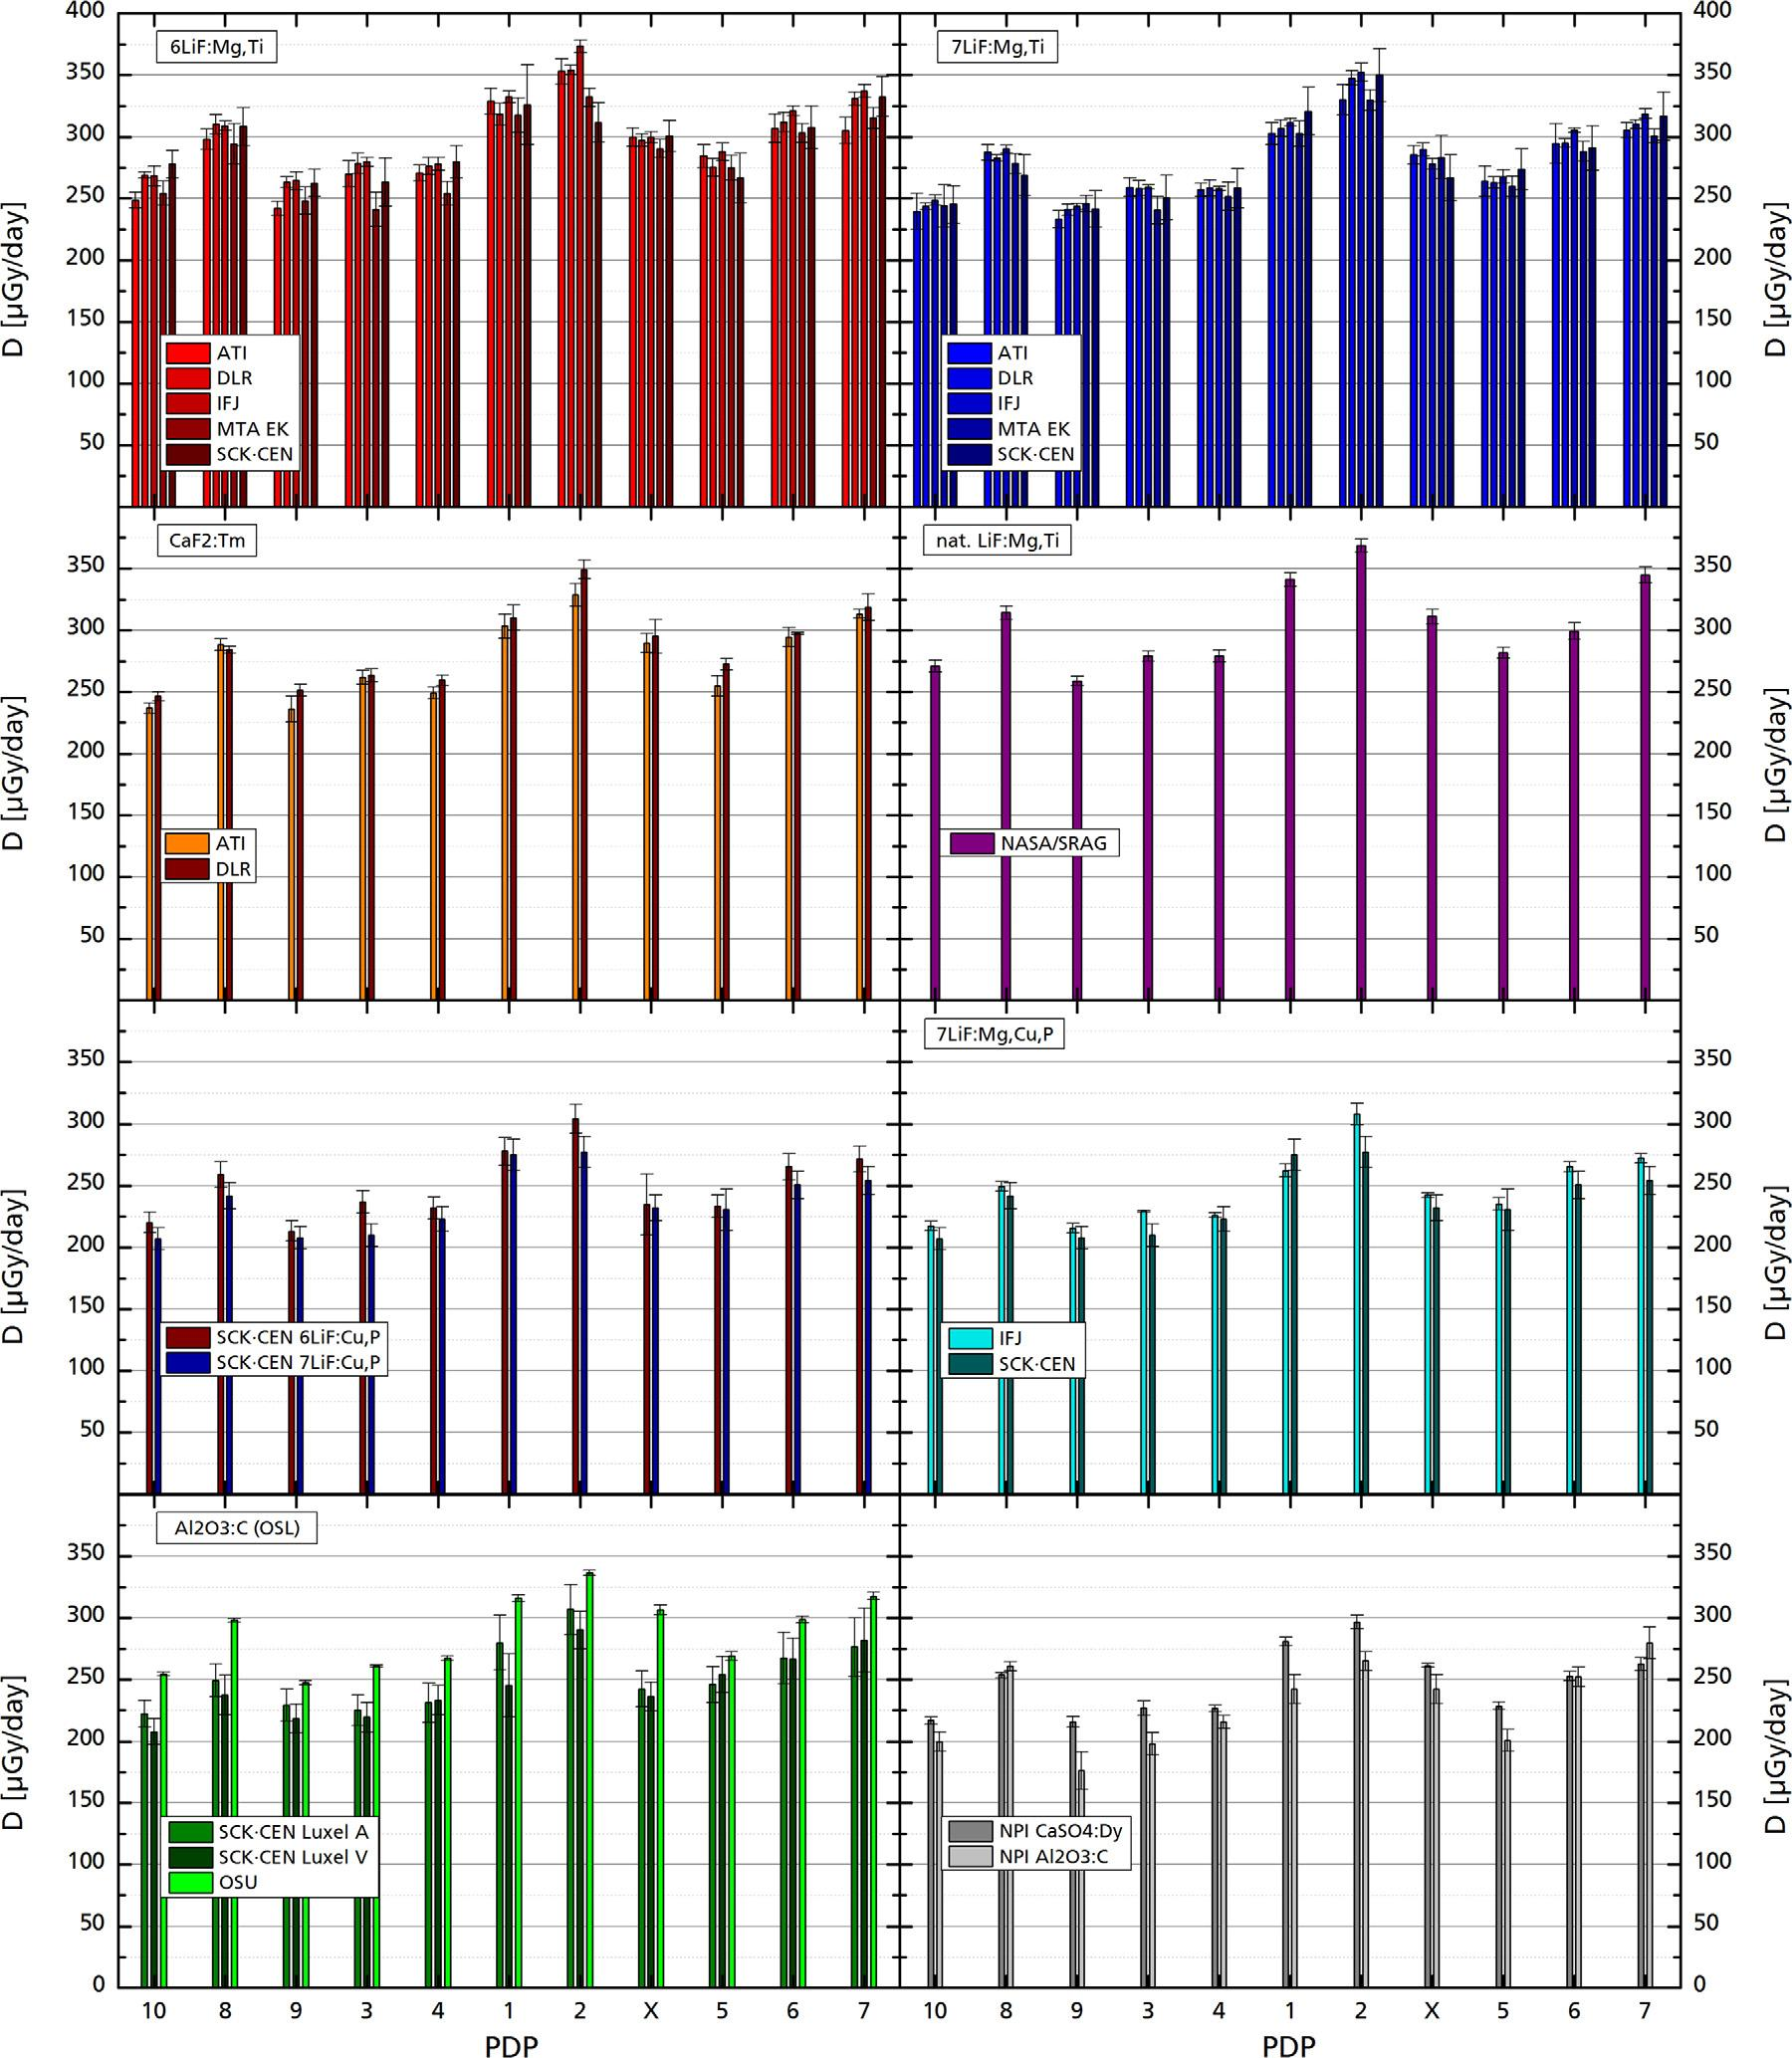
\includegraphics[height=0.65\textheight]{dosis_vysl_jednaSada.jpg}
  \caption{Naměřené dávkové příkony detektory různých materiálů. Na ose $x$ jsou čísla PDP, jejichž pořadí je založeno na poloze PDP v modulu Columbus (viz \ref{fig:columbus_rozmisteni}) \cite{dosis}.}
  \label{fig:dosis_vysl_jednaSada}
\end{figure}
\subsection{Srovnání dat z osmi sad pro jeden pasivní detektor}
Obr. \ref{fig:dosis_vysl_viceSad} zobrazuje zprůměrovaný rozsah dávkových příkonů, které byly určeny z dat $^7$LiF:Mg,Ti od několika organizací; například pro D3D2 (druhá sada DOSIS3D) je interval naměřených dávkových příkonů přibližně [250, 350] $\mu$Gy/den (lze srovnat s obr. \ref{fig:dosis_vysl_jednaSada}). Na ose $x$ je čas v letech. Obrázek dále obsahuje v horní části nadmořskou výšku ISS a četnost neutronů naměřených Oulu monitorem (viz oddíl \ref{sec:dosis_altitudeSlunecniCyklus}). Pokles dávkového příkonu z DOS1 na DOS2 (sady 1 a 2 experimentu DOSIS) byl způsoben vzrůstající sluneční aktivitou; prudký vzrůst z DOS2 na D3D1 je spojen s nárazovitým zvýšením nadmořské výšky ISS; poté se už nadmořská výška moc neměnila a pomalý pokles je tedy dán
hlavně vzrůstající sluneční aktivitou. Je zajímavé, že při D3D6 detektory obdržely jen o trochu vyšší dávky než při DOS1.
\begin{figure}[h]
  \centering
  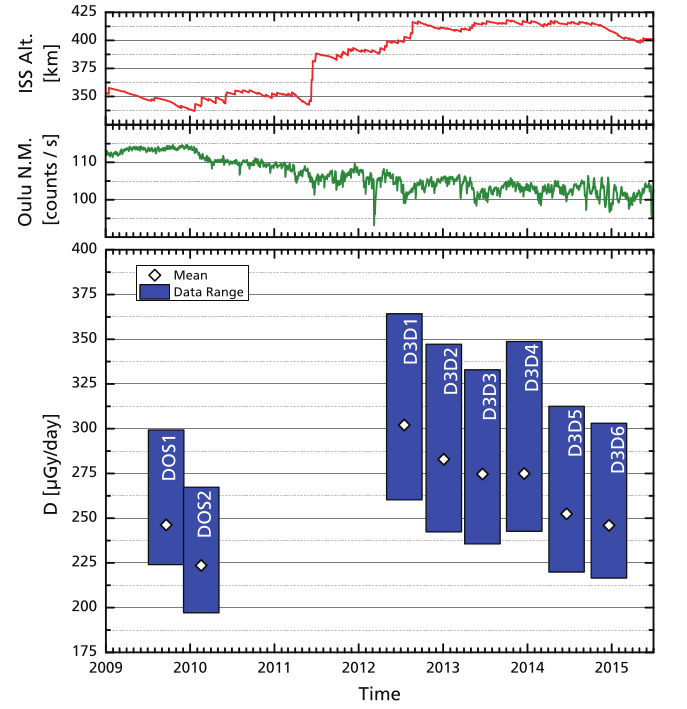
\includegraphics[width=0.65\textwidth]{dosis_vysl_viceSad.png}
  \caption{Rozsahy dávkových příkonů naměřených TLD materiálem $^7$LiF:Mg,Ti v rámci prvních osmi sad experimentů DOSIS a DOSIS3D. V horní části obrázku jsou parametry ovlivňující velikost obdržené dávky, tj. nadmořská výška ISS a četnost neutronů naměřená Oulu monitorem \cite{dosis_oulu}, která souvisí se sluneční aktivitou.}
  \label{fig:dosis_vysl_viceSad}
\end{figure}

Absorbovaná dávka z detektorů, které byly umístěny u čelní stěny vzhledem k pohybu ISS (jedná se o PDP 3, 4, 8, 9, 10), je menší než absorbovaná dávka z detektorů umístěných u zadní stěny (PDP 1, 2, 5, 6, 7, X). To je možné vysvětlit anizotropií zachycených protonů v SAA (viz oddíl \ref{sec:kosmickeZareni_anizotropie}).
\subsection{Srovnání dat pasivních a aktivních detektorů}%řešit tu vodu (absorbed dose in water)???!!!!!!!!
V tab. \ref{tab:dosis_vysl_srovnaniPassiveActive} jsou srovnány absorbované dávky určené pomocí $^7$LiF:Mg,Ti a pomocí aktivního detektoru DOSTEL-1. Data od $^7$LiF:Mg,Ti pocházejí z PDP X (viz obr.~\ref{fig:columbus_rozmisteni}), který je upevněn na boxu, v němž se nachází aktivní detektory (viz obr.~\ref{fig:dosis_activeDetectors}). Absorbované dávky aktivního detektoru byly určeny zprůměrováním dat přes časový interval odpovídající dané sadě (viz tab. \ref{tab:dosis_timeline_passive}). Hodnoty v tab. \ref{tab:dosis_vysl_srovnaniPassiveActive} představují přepočtené absorbované dávky ve vodě. Je vidět, že data z obou typů detektorů jsou ve shodě. 

Při porovnávání dat z TLD a DOSTEL je třeba brát v úvahu několik věcí. Zaprvé účinnost detekce částic nad cca 10 keV/$\mu$m u TLD klesá, zatímco u DOSTEL je v podstatě stále stoprocentní. Dále pasivní detektory byly v PDP umístěny okolo 95~\% svého měřícího cyklu, zbytek času strávily cestováním na, resp. z ISS; nicméně toto pravděpodobně nezaneslo do měření nějakou větší chybu, protože při průletu atmosférou detektory obdrží zanedbatelnou dávku.
\begin{table}[H]
  \centering
  \def\arraystretch{1}
  \footnotesize
  \begin{tabular}{lll|ll}
	\toprule
	&\multirow{2}{*}{Sada}&\multirow{2}{*}{Nadmořská výška ISS [km]}&\multicolumn{2}{c}{Absorbovaná dávka [$\mu$Gy/den]}\\
	 & & &DOSTEL-1&$^7$LiF:Mg,Ti\\
	\midrule
	DOSIS	&1&339-348&$248\pm20$&$261\pm21$\\ 
    		&2&337-349&$234\pm18$&$238\pm10$\\
    DOSIS3D	&1&397-417&$286\pm25$&$311\pm9 $\\
    		&2&407-416&$288\pm20$&$281\pm9 $\\
    		&3&407-416&$297\pm23$&$294\pm7 $\\
    		&4&413-418&$294\pm23$&$294\pm12$\\
    		&5&413-417&$279\pm22$&$262\pm7 $\\
    		&6&401-416&$256\pm20$&$256\pm7 $\\
	\bottomrule
  \end{tabular}
  \caption{Porovnání absorbovaných dávek určených pomocí aktivního detektoru DOSTEL-1 a pomocí TLD (materiál $^7$LiF:Mg,Ti), které byly umístěny v PDP X, v rámci dosud vyhodnocených sad~\cite{dosis}.}
  \label{tab:dosis_vysl_srovnaniPassiveActive}
\end{table}

Výhodou aktivních detektorů je, že dokážou rozeznat příspěvky k dávce od GCR a od zachycených protonů v SAA.


